\bta{2026}


\begin{enumerate}
	\item
	（共30分）考虑一个一维运动的自由粒子。
	\begin{enumerate}
		\item 写出定态薛定谔方程，求能量本征值、本征波函数和定态波函数（约定自由粒子波矢的取值可正可负）；
		\item 写出含时薛定谔方程的通解；
		\item 假设初始时刻局域在区间 $-a\le x\le a$ 的态为
		\[
		\psi(x,0)=\begin{cases}A,&-a\le x\le a\\0,&|x|>a\end{cases}
		\]
		其中 $A$ 和 $a$ 是正实数。波函数从 $t=0$ 开始演化，求 $\psi(x,t)$。
	\end{enumerate}

	\banswer{
	\begin{enumerate}
		\item 自由粒子 $V(x)=0$，定态薛定谔方程为
		\begin{align*}
			-\frac{\hbar^2}{2m}\frac{d^2\psi(x)}{dx^2}=E\psi(x)
		\end{align*}
		取波矢 $k\in\mathbb{R}$（可正可负），令 $E=\dfrac{\hbar^2 k^2}{2m}$，方程化为 $\psi''+k^2\psi=0$。采用约定 $\langle x|k\rangle=\dfrac{1}{\sqrt{2\pi}}e^{ikx}$，则能量本征值与本征波函数为
		\begin{align*}
			E_k=\frac{\hbar^2 k^2}{2m},\qquad \psi_k(x)=\langle x|k\rangle=\frac{1}{\sqrt{2\pi}}e^{ikx},\qquad k\in\mathbb{R}
		\end{align*}
		每一个 $E_k>0$ 对应 $k=\pm\sqrt{2mE}/\hbar$ 两个行波解，即二重简并。定态波函数为
		\begin{align*}
			\Psi_k(x,t)=\psi_k(x)e^{-iE_k t/\hbar}=\frac{1}{\sqrt{2\pi}}\exp\!\left(ikx-\frac{i\hbar k^2}{2m}t\right)
		\end{align*}

		\item 含时薛定谔方程 $i\hbar\dfrac{\partial}{\partial t}\Psi(x,t)=-\dfrac{\hbar^2}{2m}\dfrac{\partial^2}{\partial x^2}\Psi(x,t)$ 的通解为各定态的 Fourier 积分叠加：
		\begin{align*}
			\Psi(x,t)=\frac{1}{\sqrt{2\pi}}\int_{-\infty}^{+\infty}c(k)\exp\!\left(ikx-\frac{i\hbar k^2}{2m}t\right)dk
		\end{align*}
		其中展开系数由初态决定，$c(k)=\langle k|\Psi(0)\rangle=\dfrac{1}{\sqrt{2\pi}}\displaystyle\int_{-\infty}^{+\infty}\Psi(x,0)e^{-ikx}\,dx$。

		\item 先由归一化确定 $A$：
		\begin{align*}
			1=\int_{-\infty}^{+\infty}|\psi(x,0)|^2\,dx=A^2\int_{-a}^{a}dx=2aA^2
		\end{align*}
		故归一化要求 $A=\dfrac{1}{\sqrt{2a}}$。以下推导对一般正实数 $A$ 均成立。

		计算初态的 Fourier 变换：
		\begin{align*}
			c(k)&=\frac{1}{\sqrt{2\pi}}\int_{-a}^{a}Ae^{-ikx}\,dx=\frac{A}{\sqrt{2\pi}}\cdot\frac{e^{ika}-e^{-ika}}{ik}\\
			&=\frac{A}{\sqrt{2\pi}}\cdot\frac{2\sin(ka)}{k}
		\end{align*}
		代入通解，得
		\begin{align*}
			\psi(x,t)&=\frac{1}{\sqrt{2\pi}}\int_{-\infty}^{+\infty}\frac{A}{\sqrt{2\pi}}\cdot\frac{2\sin(ka)}{k}\exp\!\left(ikx-\frac{i\hbar k^2}{2m}t\right)dk\\
			&=\frac{A}{\pi}\int_{-\infty}^{+\infty}\frac{\sin(ka)}{k}\exp\!\left(ikx-\frac{i\hbar k^2}{2m}t\right)dk
		\end{align*}

		等价地，利用自由粒子传播子 $K(x,t;x',0)=\sqrt{\dfrac{m}{2\pi i\hbar t}}\exp\!\left(\dfrac{im(x-x')^2}{2\hbar t}\right)$，可写为对初态支区间 $[-a,a]$ 的积分：
		\begin{align*}
			\psi(x,t)=\int_{-a}^{a}K(x,t;x',0)\psi(x',0)\,dx'=A\sqrt{\frac{m}{2\pi i\hbar t}}\int_{-a}^{a}\exp\!\left(\frac{im(x-x')^2}{2\hbar t}\right)dx'
		\end{align*}

		验证初条件：当 $t\to 0^+$ 时，
		\begin{align*}
			\psi(x,0^+)&=\frac{A}{\pi}\int_{-\infty}^{+\infty}\frac{\sin(ka)}{k}e^{ikx}\,dk=\frac{A}{2\pi}\int_{-\infty}^{+\infty}\int_{-a}^{a}e^{ik(x-x')}\,dx'\,dk\\
			&=A\int_{-a}^{a}\delta(x-x')\,dx'=\begin{cases}A,&|x|<a\\0,&|x|>a\end{cases}
		\end{align*}
		与给定的初态一致（端点 $x=\pm a$ 处取 Fourier 收敛值 $A/2$）。
	\end{enumerate}
	}

	\item
	（共30分）质量 $m$、电荷 $q$ 的粒子被束缚在三维各向同性谐振子势场中，
	\[
	V(x,y,z)=\frac{1}{2}m\omega_0^2(x^2+y^2+z^2),\qquad \omega_0=\sqrt{\frac{k}{m}}
	\]
	\begin{enumerate}
		\item 写出 $H_0$ 的完整表达式，求本征能谱 $E_N$，并分析 $E_N$ 的简并度；
		\item 写出基态波函数的具体形式（无需归一化），并说明其量子数；
		\item 额外受到沿 $x$ 方向均匀交变电场 $E_x(t)=E_0\cos(\omega t)$，写出总含时 Hamilton 量；$E_0$ 很小，推导 $|\psi_i\rangle$ 到 $|\psi_f\rangle$ 的选择定则。
	\end{enumerate}

	提示：$x=\sqrt{\dfrac{\hbar}{2m\omega}}(a_x+a_x^{\dagger})$。

	\banswer{
	\begin{enumerate}
		\item 三维各向同性谐振子可分离为三个频率均为 $\omega_0$ 的一维谐振子：
		\begin{align*}
			H_0=\frac{\hat{p}_x^2+\hat{p}_y^2+\hat{p}_z^2}{2m}+\frac{1}{2}m\omega_0^2(x^2+y^2+z^2)
		\end{align*}
		引入各方向产生湮灭算符后，
		\begin{align*}
			H_0=\hbar\omega_0\left(N_x+N_y+N_z+\frac{3}{2}\right)
		\end{align*}
		令 $N=N_x+N_y+N_z$，本征能谱为
		\begin{align*}
			E_N=\hbar\omega_0\left(N+\frac{3}{2}\right),\qquad N=0,1,2,\ldots
		\end{align*}
		简并度等于方程 $n_x+n_y+n_z=N$ 的非负整数解个数：
		\begin{align*}
			g_N=\binom{N+2}{2}=\frac{(N+1)(N+2)}{2}
		\end{align*}

		\item 基态对应 $n_x=n_y=n_z=0$，即 $N=0$，能量 $E_0=\dfrac{3}{2}\hbar\omega_0$。波函数为三个一维基态之积（无需归一化）：
		\begin{align*}
			\psi_0(x,y,z)\propto\exp\!\left(-\frac{m\omega_0}{2\hbar}(x^2+y^2+z^2)\right)=\exp\!\left(-\frac{m\omega_0 r^2}{2\hbar}\right)
		\end{align*}
		这是仅依赖 $r$ 的三维 Gauss 型 $s$ 态，量子数为 $n_x=n_y=n_z=0$，总量子数 $N=0$，轨道角动量量子数 $l=0$，磁量子数 $m_l=0$，非简并（$g_0=1$）。

		\item 电荷 $q$ 在电场 $\vec{E}=E_0\cos(\omega t)\hat{x}$ 中的相互作用能为 $-q\vec{E}\cdot\vec{r}$，故总含时 Hamilton 量为
		\begin{align*}
			H(t)=H_0-qE_0 x\cos(\omega t)
		\end{align*}
		微扰 $H'(t)=-qE_0 x\cos(\omega t)$。

		关于提示中的频率：坐标算符的展开 $x=\sqrt{\dfrac{\hbar}{2m\omega}}(a_x+a_x^{\dagger})$ 中的 $\omega$ 必须取系统自身的振子频率 $\omega_0$，即 $x=\sqrt{\dfrac{\hbar}{2m\omega_0}}(a_x+a_x^{\dagger})$；外场频率 $\omega$ 只出现在 $\cos(\omega t)$ 中，二者不可混淆。

		矩阵元为
		\begin{align*}
			\langle f|x|i\rangle=\sqrt{\frac{\hbar}{2m\omega_0}}\langle n_x',n_y',n_z'|(a_x+a_x^{\dagger})|n_x,n_y,n_z\rangle
		\end{align*}
		由于 $a_x|n_x\rangle=\sqrt{n_x}|n_x-1\rangle$，$a_x^{\dagger}|n_x\rangle=\sqrt{n_x+1}|n_x+1\rangle$，且 $y,z$ 方向需正交守恒，矩阵元非零的条件为
		\begin{align*}
			\Delta n_x=n_x'-n_x=\pm1,\qquad \Delta n_y=0,\qquad \Delta n_z=0
		\end{align*}
		此即选择定则。再由含时微扰论，$\cos(\omega t)=\dfrac{1}{2}(e^{i\omega t}+e^{-i\omega t})$ 在长时间极限下给出能量守恒：
		\begin{align*}
			E_f-E_i=\pm\hbar\omega
		\end{align*}
		其中 $E_f-E_i=+\hbar\omega$ 对应吸收（$\Delta n_x=+1$），$E_f-E_i=-\hbar\omega$ 对应受激发射（$\Delta n_x=-1$）。由于能级间隔固定为 $\hbar\omega_0$，共振条件即 $\omega=\omega_0$。
	\end{enumerate}
	}

	\item
	（共30分）三维空间中自旋 $1/2$ 单粒子系统，单位矩阵 $E$ 和 Pauli 矩阵为
	\[
	E=\begin{pmatrix}1&0\\0&1\end{pmatrix},\qquad
	\sigma_x=\begin{pmatrix}0&1\\1&0\end{pmatrix},\qquad
	\sigma_y=\begin{pmatrix}0&-i\\i&0\end{pmatrix},\qquad
	\sigma_z=\begin{pmatrix}1&0\\0&-1\end{pmatrix}
	\]
	\begin{enumerate}
		\item 计算 $[\sigma_x,\sigma_y]$，$[\sigma_y,\sigma_z]$，$[\sigma_z,\sigma_x]$，以及 $\{\sigma_x,\sigma_y\}$，$\{\sigma_y,\sigma_z\}$，$\{\sigma_z,\sigma_x\}$；
		\item 用 $[E,\sigma_x,\sigma_y,\sigma_z]$ 展开 $e^{i\theta\sigma_z}=aE+b\sigma_x+c\sigma_y+d\sigma_z$，求 $a,b,c,d$；
		\item 沿 $z$ 方向磁场 $B$，Hamilton 量 $H=B\sigma_z$。$t=0$ 时 $|\psi\rangle=\dfrac{1}{\sqrt{2}}\begin{pmatrix}1\\1\end{pmatrix}$。求 $|\psi(t)\rangle$ 和三个 Pauli 算符的期望值。
	\end{enumerate}

	提示：$e^{i\theta\sigma_z}=\displaystyle\sum_{n=0}^{\infty}\dfrac{(i\theta\sigma_z)^n}{n!}$。

	\banswer{
	\begin{enumerate}
		\item 直接矩阵相乘。对 $[\sigma_x,\sigma_y]$：
		\begin{align*}
			\sigma_x\sigma_y&=\begin{pmatrix}0&1\\1&0\end{pmatrix}\begin{pmatrix}0&-i\\i&0\end{pmatrix}=\begin{pmatrix}i&0\\0&-i\end{pmatrix}=i\sigma_z\\
			\sigma_y\sigma_x&=\begin{pmatrix}0&-i\\i&0\end{pmatrix}\begin{pmatrix}0&1\\1&0\end{pmatrix}=\begin{pmatrix}-i&0\\0&i\end{pmatrix}=-i\sigma_z
		\end{align*}
		故 $[\sigma_x,\sigma_y]=2i\sigma_z$。轮换得
		\begin{align*}
			[\sigma_y,\sigma_z]=2i\sigma_x,\qquad [\sigma_z,\sigma_x]=2i\sigma_y
		\end{align*}
		即统一形式 $[\sigma_i,\sigma_j]=2i\epsilon_{ijk}\sigma_k$。

		反对易子：
		\begin{align*}
			\{\sigma_x,\sigma_y\}=\sigma_x\sigma_y+\sigma_y\sigma_x=i\sigma_z+(-i\sigma_z)=0
		\end{align*}
		同理
		\begin{align*}
			\{\sigma_y,\sigma_z\}=0,\qquad \{\sigma_z,\sigma_x\}=0
		\end{align*}
		即不同 Pauli 矩阵两两反对易，$\{\sigma_i,\sigma_j\}=2\delta_{ij}E$。

		\item 由 $\sigma_z^2=E$，按 Taylor 展开分离奇偶次幂：
		\begin{align*}
			e^{i\theta\sigma_z}&=\sum_{n=0}^{\infty}\frac{(i\theta)^n\sigma_z^n}{n!}=\sum_{k=0}^{\infty}\frac{(i\theta)^{2k}}{(2k)!}E+\sum_{k=0}^{\infty}\frac{(i\theta)^{2k+1}}{(2k+1)!}\sigma_z\\
			&=\left(\sum_{k=0}^{\infty}\frac{(-1)^k\theta^{2k}}{(2k)!}\right)E+i\left(\sum_{k=0}^{\infty}\frac{(-1)^k\theta^{2k+1}}{(2k+1)!}\right)\sigma_z\\
			&=\cos\theta\,E+i\sin\theta\,\sigma_z
		\end{align*}
		与 $aE+b\sigma_x+c\sigma_y+d\sigma_z$ 比较，得
		\begin{align*}
			a=\cos\theta,\qquad b=0,\qquad c=0,\qquad d=i\sin\theta
		\end{align*}

		\item $H=B\sigma_z$ 与时间无关，时间演化算符为
		\begin{align*}
			U(t)=e^{-iHt/\hbar}=e^{-i(Bt/\hbar)\sigma_z}=\cos\!\left(\frac{Bt}{\hbar}\right)E-i\sin\!\left(\frac{Bt}{\hbar}\right)\sigma_z
		\end{align*}
		即对角形式 $U(t)=\operatorname{diag}(e^{-iBt/\hbar},e^{iBt/\hbar})$。作用于初态：
		\begin{align*}
			|\psi(t)\rangle=U(t)|\psi(0)\rangle=\frac{1}{\sqrt{2}}\begin{pmatrix}e^{-iBt/\hbar}\\e^{iBt/\hbar}\end{pmatrix}
		\end{align*}

		计算期望值。对 $\sigma_x$：
		\begin{align*}
			\langle\sigma_x\rangle&=\frac{1}{2}\begin{pmatrix}e^{iBt/\hbar}&e^{-iBt/\hbar}\end{pmatrix}\begin{pmatrix}0&1\\1&0\end{pmatrix}\begin{pmatrix}e^{-iBt/\hbar}\\e^{iBt/\hbar}\end{pmatrix}\\
			&=\frac{1}{2}(e^{2iBt/\hbar}+e^{-2iBt/\hbar})=\cos\!\left(\frac{2Bt}{\hbar}\right)
		\end{align*}
		对 $\sigma_y$：
		\begin{align*}
			\langle\sigma_y\rangle&=\frac{1}{2}\begin{pmatrix}e^{iBt/\hbar}&e^{-iBt/\hbar}\end{pmatrix}\begin{pmatrix}0&-i\\i&0\end{pmatrix}\begin{pmatrix}e^{-iBt/\hbar}\\e^{iBt/\hbar}\end{pmatrix}\\
			&=\frac{1}{2}(-ie^{2iBt/\hbar}+ie^{-2iBt/\hbar})=\frac{1}{2}\cdot 2\sin\!\left(\frac{2Bt}{\hbar}\right)=\sin\!\left(\frac{2Bt}{\hbar}\right)
		\end{align*}
		对 $\sigma_z$：
		\begin{align*}
			\langle\sigma_z\rangle=\frac{1}{2}(|e^{-iBt/\hbar}|^2-|e^{iBt/\hbar}|^2)=\frac{1}{2}(1-1)=0
		\end{align*}
		故
		\begin{align*}
			\langle\sigma_x\rangle=\cos\!\left(\frac{2Bt}{\hbar}\right),\qquad \langle\sigma_y\rangle=\sin\!\left(\frac{2Bt}{\hbar}\right),\qquad \langle\sigma_z\rangle=0
		\end{align*}
		自旋期望矢量在 $xOy$ 平面内以角频率 $2B/\hbar$ 进动，模长恒为 $1$。
	\end{enumerate}
	}

	\item
	（共30分）对于一维谐振子势 $V(x)$，基态能量为 $E_0$。
	\begin{enumerate}
		\item 画出基态波函数示意图；
		\item 对于基态，画出经典允许区和禁戒区，说明波函数在两区的凹凸性；
		\item 已知误差函数 $\operatorname{erf}(x)=\dfrac{2}{\sqrt{\pi}}\displaystyle\int_0^x e^{-\xi^2}\,d\xi$。用 $\operatorname{erf}$ 表示基态中粒子处于禁戒区的几率。
	\end{enumerate}

	\banswer{
	\begin{enumerate}
		\item 设谐振子势 $V(x)=\dfrac{1}{2}m\Omega^2 x^2$，基态能量 $E_0=\dfrac{1}{2}\hbar\Omega$，特征长度 $x_t=\sqrt{\dfrac{\hbar}{m\Omega}}$。基态波函数为无节点的偶 Gauss 函数：
		\begin{align*}
			\psi_0(x)=\left(\frac{m\Omega}{\pi\hbar}\right)^{1/4}e^{-x^2/(2x_t^2)}
		\end{align*}
		示意图如下（正值、偶对称、无节点、向两侧指数衰减）：
		\begin{center}
		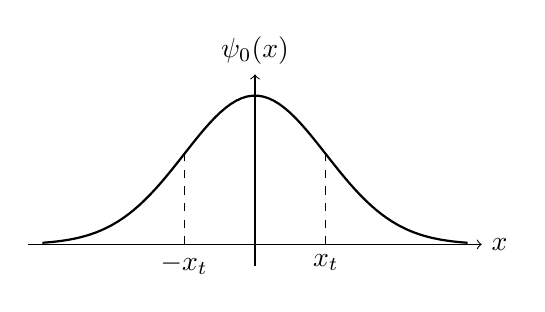
\begin{tikzpicture}[scale=0.9]
			\draw[->] (-3.2,0)--(3.2,0) node[right]{$x$};
			\draw[->] (0,-0.3)--(0,2.4) node[above]{$\psi_0(x)$};
			\draw[thick,domain=-3:3,samples=80] plot (\x,{2.1*exp(-\x*\x/2)});
			\draw[dashed] (-1,0) node[below]{$-x_t$}--(-1,{2.1*exp(-0.5)});
			\draw[dashed] (1,0) node[below]{$x_t$}--(1,{2.1*exp(-0.5)});
		\end{tikzpicture}
		\end{center}

		\item 经典转折点由 $V(x)=E_0$ 确定：$\dfrac{1}{2}m\Omega^2 x^2=\dfrac{1}{2}\hbar\Omega$，即 $x=\pm x_t$。

		\begin{center}
		\begin{tikzpicture}[scale=0.9]
			\fill[gray!25] (-3,0) rectangle (-1,0.5);
			\fill[gray!25] (1,0) rectangle (3,0.5);
			\draw[->] (-3.2,0)--(3.2,0) node[right]{$x$};
			\draw[->] (0,-0.3)--(0,2.6) node[above]{$V,E$};
			\draw[thick,domain=-2.2:2.2,samples=60] plot (\x,{0.5*\x*\x});
			\draw[thick] (-3,0.5)--(3,0.5) node[right]{$E_0=\frac{1}{2}\hbar\Omega$};
			\draw[dashed] (-1,0) node[below]{$-x_t$}--(-1,0.5);
			\draw[dashed] (1,0) node[below]{$x_t$}--(1,0.5);
			\node at (0,0.25){\small 允许区};
			\node at (-2,0.25){\small 禁戒区};
			\node at (2,0.25){\small 禁戒区};
		\end{tikzpicture}
		\end{center}

		由定态方程 $\psi_0''=\dfrac{2m}{\hbar^2}(V-E_0)\psi_0$，且基态 $\psi_0(x)>0$ 处处成立，凹凸性完全由 $V-E_0$ 的符号决定：
		\begin{align*}
			\psi_0''\begin{cases}<0,&|x|<x_t\ \text{（经典允许区，}V<E_0\text{，曲线下凸即开口向下）}\\>0,&|x|>x_t\ \text{（经典禁戒区，}V>E_0\text{，曲线上凸即开口向上）}\end{cases}
		\end{align*}
		即允许区内 $\psi_0''<0$，曲线呈峰形向下弯曲；禁戒区内 $\psi_0''>0$，曲线向上翘起并指数衰减趋于零。

		\item 基态几率密度 $|\psi_0(x)|^2=\sqrt{\dfrac{m\Omega}{\pi\hbar}}\,e^{-x^2/x_t^2}$。禁戒区几率为
		\begin{align*}
			P_{\text{禁}}=2\int_{x_t}^{+\infty}|\psi_0(x)|^2\,dx=\frac{2}{\sqrt{\pi}\,x_t}\int_{x_t}^{+\infty}e^{-x^2/x_t^2}\,dx
		\end{align*}
		令 $\xi=x/x_t$：
		\begin{align*}
			P_{\text{禁}}=\frac{2}{\sqrt{\pi}}\int_1^{+\infty}e^{-\xi^2}\,d\xi=\frac{2}{\sqrt{\pi}}\left(\frac{\sqrt{\pi}}{2}-\int_0^1 e^{-\xi^2}\,d\xi\right)=1-\operatorname{erf}(1)
		\end{align*}
		即
		\begin{align*}
			P_{\text{禁}}=1-\operatorname{erf}(1)=\operatorname{erfc}(1)\approx 0.1573
		\end{align*}
		约有 $15.73\%$ 的几率在经典禁戒区中找到粒子，这源于量子穿透效应，即基态波函数在经典禁戒区内仍有非零的指数衰减尾巴。
	\end{enumerate}
	}

	\item
	（共30分）考虑处于磁场 $\vec{B}=\nabla\times\vec{A}$ 中的无自旋带电粒子，Hamilton 量为
	\[
	H=\frac{1}{2}\left(\vec{p}-\frac{q\vec{A}}{c}\right)^2
	\]
	均匀强磁场沿 $z$ 方向 $\vec{B}=B_0\hat{e}_z$。
	\begin{enumerate}
		\item 取 $\vec{A}=-B_0 y\,\hat{e}_x$，证明 $p_x$ 和 $p_z$ 是守恒量，并求本征能级；
		\item 设 $\vec{A}=(-B_0 y,0,0)$，$\vec{A}_1=\dfrac{1}{2}\vec{B}\times\vec{r}=\left(-\dfrac{B_0 y}{2},\dfrac{B_0 x}{2},0\right)$。在 $\vec{A}$ 到 $\vec{A}_1$ 的规范变换下保持薛定谔方程不变，求波函数变换；
		\item 柱坐标 $(\rho,\varphi,z)$，磁场仅存在于 $\rho<a$ 的很小柱形区域，通量为 $\phi$，$\rho>a$ 无磁场，令 $a\to 0$；$\rho\neq 0$ 处 $\vec{A}=\nabla f$，求 $f$。
	\end{enumerate}

	提示：柱坐标梯度 $\nabla f=\dfrac{\partial f}{\partial \rho}\hat{e}_{\rho}+\dfrac{1}{\rho}\dfrac{\partial f}{\partial\varphi}\hat{e}_{\varphi}+\dfrac{\partial f}{\partial z}\hat{e}_z$。

	\banswer{
	\begin{enumerate}
		\item 题面所印 Hamilton 量 $H=\dfrac{1}{2}\left(\vec{p}-\dfrac{q\vec{A}}{c}\right)^2$ 对应于取质量 $m=1$ 的单位制；以下恢复一般质量 $m$，采用标准形式
		\begin{align*}
			H=\frac{1}{2m}\left(\vec{p}-\frac{q\vec{A}}{c}\right)^2
		\end{align*}
		取 $\vec{A}=(-B_0 y,0,0)$（满足 $\nabla\times\vec{A}=B_0\hat{e}_z$），则
		\begin{align*}
			H=\frac{1}{2m}\left[\left(p_x+\frac{qB_0}{c}y\right)^2+p_y^2+p_z^2\right]
		\end{align*}
		$H$ 中不显含坐标 $x,z$，故
		\begin{align*}
			[p_x,H]=0,\qquad [p_z,H]=0
		\end{align*}
		即 $p_x,p_z$ 为守恒量（运动常数），可与 $H$ 取共同本征态。

		取本征函数 $\psi(x,y,z)=e^{i(k_x x+k_z z)}\varphi(y)$，代入定态方程得 $y$ 方向方程：
		\begin{align*}
			\left[-\frac{\hbar^2}{2m}\frac{d^2}{dy^2}+\frac{1}{2m}\left(\hbar k_x+\frac{qB_0}{c}y\right)^2\right]\varphi(y)=\left(E-\frac{\hbar^2 k_z^2}{2m}\right)\varphi(y)
		\end{align*}
		这是关于 $y$ 的谐振子，平衡位置（回旋中心）
		\begin{align*}
			y_0=-\frac{c\hbar k_x}{qB_0}
		\end{align*}
		回旋频率
		\begin{align*}
			\omega_c=\frac{|q|B_0}{mc}
		\end{align*}
		故本征能级（Landau 能级）为
		\begin{align*}
			E_{n,k_z}=\hbar\omega_c\left(n+\frac{1}{2}\right)+\frac{\hbar^2 k_z^2}{2m},\qquad n=0,1,2,\ldots
		\end{align*}
		能量与 $k_x$ 无关，$k_x$（即回旋中心 $y_0$ 的取值）带来高度简并。

		\item 两矢势逐分量相减：
		\begin{align*}
			\vec{A}_1-\vec{A}=\left(-\frac{B_0 y}{2},\frac{B_0 x}{2},0\right)-(-B_0 y,0,0)=\left(\frac{B_0 y}{2},\frac{B_0 x}{2},0\right)
		\end{align*}
		取规范函数
		\begin{align*}
			\chi=\frac{B_0 xy}{2}
		\end{align*}
		则 $\nabla\chi=\left(\dfrac{B_0 y}{2},\dfrac{B_0 x}{2},0\right)=\vec{A}_1-\vec{A}$，即 $\vec{A}_1=\vec{A}+\nabla\chi$，确为规范变换。

		规范变换下保持薛定谔方程不变，波函数需乘以相位因子：
		\begin{align*}
			\psi_{A_1}=\exp\!\left(\frac{iq\chi}{\hbar c}\right)\psi_A=\exp\!\left(\frac{iqB_0 xy}{2\hbar c}\right)\psi_A
		\end{align*}

		\item 题中通量原印为 $\phi$；为避免与柱坐标方位角 $\varphi$ 混淆，以下将磁通量改记为 $\Phi$（即 $\Phi\equiv\phi$）。将磁通 $\Phi$ 约束在 $\rho<a$ 的细柱内，$\rho>a$ 处 $\vec{B}=0$。由 Stokes 定理，对半径 $\rho>a$ 的回路：
		\begin{align*}
			\oint \vec{A}\cdot d\vec{l}=\int \vec{B}\cdot d\vec{S}=\Phi
		\end{align*}
		由轴对称性 $\vec{A}=A_{\varphi}(\rho)\hat{e}_{\varphi}$，故 $A_{\varphi}\cdot 2\pi\rho=\Phi$，即
		\begin{align*}
			A_{\varphi}=\frac{\Phi}{2\pi\rho},\qquad \vec{A}=\frac{\Phi}{2\pi\rho}\hat{e}_{\varphi}\quad(\rho>a)
		\end{align*}
		令 $a\to 0$，上式在 $\rho\neq 0$ 处成立。设 $\vec{A}=\nabla f$，由柱坐标梯度公式，因 $A_{\rho}=A_z=0$，$f$ 与 $\rho,z$ 无关，仅
		\begin{align*}
			\frac{1}{\rho}\frac{\partial f}{\partial\varphi}=A_{\varphi}=\frac{\Phi}{2\pi\rho}
		\end{align*}
		积分得
		\begin{align*}
			f=\frac{\Phi\varphi}{2\pi}+\text{常数}
		\end{align*}
		注意 $\varphi$ 是方位角，绕原点一周 $\varphi\to\varphi+2\pi$ 时 $f\to f+\Phi$，故 $f$ 是全局多值函数（这正反映出 $\rho=0$ 处有磁通奇点，该区域 $\vec{B}\neq 0$，不能整体取 $\vec{A}=\nabla f$）。带电粒子绕磁通一周获得的 Aharonov--Bohm 相位为
		\begin{align*}
			\Delta\gamma=\frac{q}{\hbar c}\oint\vec{A}\cdot d\vec{l}=\frac{q\Phi}{\hbar c}
		\end{align*}
		即使粒子始终运动在 $\vec{B}=0$ 的区域，该相位仍可观测，即 Aharonov--Bohm 效应。
	\end{enumerate}
	}

\end{enumerate}
